\documentclass[10pt,journal,compsoc]{IEEEtran}
% IEEE Transactions on Knowledge and Data Engineering -- regular paper.
% IEEE Computer Society journal template (IEEEtran.cls, compsoc option).
\usepackage[T1]{fontenc}
\usepackage[nocompress]{cite}
\usepackage{amsmath,amssymb,amsfonts}
\usepackage{algorithm}
\usepackage{algpseudocode}
\usepackage{graphicx}
\usepackage{booktabs}
\usepackage{multirow}
\usepackage{xcolor}
\usepackage{tikz}
\usetikzlibrary{arrows.meta,positioning,fit,calc}
\usepackage[hidelinks]{hyperref}

% every result number is a macro generated by make_figures.py from experiments/results
% generated by make_figures.py from experiments/results -- do not edit
\newcommand{\Nadmmcols}{16.8}
\newcommand{\Nadmmcolskeys}{51.8}
\newcommand{\Nadmocols}{51.8}
\newcommand{\Nadmocolskeys}{65.5}
\newcommand{\Nadmqcols}{20.0}
\newcommand{\Nadmqcolskeys}{52.7}
\newcommand{\Nadmscols}{60.0}
\newcommand{\Nadmscolskeys}{70.0}
\newcommand{\Nadvmlinear}{0.0}
\newcommand{\Nadvmlinearhi}{7.1}
\newcommand{\Nadvmlinearrefusals}{5.1}
\newcommand{\Nadvmpairwise}{24.0}
\newcommand{\Nadvmpairwisehi}{37.4}
\newcommand{\Nadvmpairwiserefusals}{5.0}
\newcommand{\Nadvmpurpose}{98.0}
\newcommand{\Nadvmpurposehi}{99.6}
\newcommand{\Nadvmpurposerefusals}{0.2}
\newcommand{\Nadvmstateless}{10.0}
\newcommand{\Nadvmstatelesshi}{21.4}
\newcommand{\Nadvmstatelessrefusals}{2.2}
\newcommand{\Nadvmstrict}{0.0}
\newcommand{\Nadvmstricthi}{7.1}
\newcommand{\Nadvmstrictrefusals}{5.4}
\newcommand{\Nadvnm}{50}
\newcommand{\Nadvno}{25}
\newcommand{\Nadvolinear}{0.0}
\newcommand{\Nadvolinearhi}{13.3}
\newcommand{\Nadvolinearrefusals}{3.8}
\newcommand{\Nadvopairwise}{24.0}
\newcommand{\Nadvopairwisehi}{43.4}
\newcommand{\Nadvopairwiserefusals}{3.0}
\newcommand{\Nadvopurpose}{88.0}
\newcommand{\Nadvopurposehi}{95.8}
\newcommand{\Nadvopurposerefusals}{0.0}
\newcommand{\Nadvostateless}{12.0}
\newcommand{\Nadvostatelesshi}{30.0}
\newcommand{\Nadvostatelessrefusals}{2.9}
\newcommand{\Naucdriftbreadth}{0.71}
\newcommand{\Naucdriftbreadthq}{0.71}
\newcommand{\Naucdriftcell}{0.50}
\newcommand{\Naucdriftcellq}{0.50}
\newcommand{\Naucdriftdrift}{0.98}
\newcommand{\Naucdriftdriftq}{0.97}
\newcommand{\Naucdriftqueries}{0.53}
\newcommand{\Naucdriftrowledger}{0.71}
\newcommand{\Naucdriftsqlguardcount}{0.71}
\newcommand{\Naucenumerationbreadth}{1.00}
\newcommand{\Naucenumerationbreadthq}{0.94}
\newcommand{\Naucenumerationcell}{0.50}
\newcommand{\Naucenumerationcellq}{0.50}
\newcommand{\Naucenumerationdrift}{0.35}
\newcommand{\Naucenumerationdriftq}{0.35}
\newcommand{\Naucenumerationqueries}{0.61}
\newcommand{\Naucenumerationrowledger}{1.00}
\newcommand{\Naucenumerationsqlguardcount}{0.99}
\newcommand{\Naucsmallcellbreadth}{0.47}
\newcommand{\Naucsmallcellbreadthq}{0.47}
\newcommand{\Naucsmallcellcell}{0.92}
\newcommand{\Naucsmallcellcellq}{1.00}
\newcommand{\Naucsmallcelldrift}{0.44}
\newcommand{\Naucsmallcelldriftq}{0.44}
\newcommand{\Naucsmallcellqueries}{0.56}
\newcommand{\Naucsmallcellrowledger}{0.52}
\newcommand{\Naucsmallcellsqlguardcount}{0.60}
\newcommand{\Nauctrackerthreebreadth}{0.47}
\newcommand{\Nauctrackerthreebreadthq}{0.47}
\newcommand{\Nauctrackerthreecell}{0.48}
\newcommand{\Nauctrackerthreecellq}{0.50}
\newcommand{\Nauctrackerthreedrift}{0.33}
\newcommand{\Nauctrackerthreedriftq}{0.33}
\newcommand{\Nauctrackerthreequeries}{0.51}
\newcommand{\Nauctrackerthreerowledger}{0.41}
\newcommand{\Nauctrackerthreesqlguardcount}{0.57}
\newcommand{\Nauctrackerbreadth}{0.47}
\newcommand{\Nauctrackerbreadthq}{0.47}
\newcommand{\Nauctrackercell}{0.92}
\newcommand{\Nauctrackercellq}{0.49}
\newcommand{\Nauctrackerdrift}{0.33}
\newcommand{\Nauctrackerdriftq}{0.33}
\newcommand{\Nauctrackerqueries}{0.54}
\newcommand{\Nauctrackerrowledger}{0.46}
\newcommand{\Nauctrackersqlguardcount}{0.59}
\newcommand{\Nbenignleak}{13.8}
\newcommand{\Nbenignleakn}{55}
\newcommand{\Ncolsmcols}{3.7}
\newcommand{\Ncolsmcolskeys}{7.4}
\newcommand{\Ncolsmesc}{7.5}
\newcommand{\Ncolsmfull}{72.5}
\newcommand{\Ncolsmgold}{4.6}
\newcommand{\Ncolsmtables}{27.1}
\newcommand{\Ncolsocols}{4.4}
\newcommand{\Ncolsocolskeys}{7.3}
\newcommand{\Ncolsoesc}{7.3}
\newcommand{\Ncolsofull}{72.5}
\newcommand{\Ncolsogold}{4.6}
\newcommand{\Ncolsotables}{27.8}
\newcommand{\Ncolsqcols}{3.8}
\newcommand{\Ncolsqcolskeys}{7.9}
\newcommand{\Ncolsqesc}{8.0}
\newcommand{\Ncolsqfull}{72.5}
\newcommand{\Ncolsqgold}{4.7}
\newcommand{\Ncolsqtables}{31.9}
\newcommand{\Ncolsscols}{4.4}
\newcommand{\Ncolsscolskeys}{7.3}
\newcommand{\Ncolssesc}{7.4}
\newcommand{\Ncolssfull}{72.5}
\newcommand{\Ncolssgold}{4.6}
\newcommand{\Ncolsstables}{28.0}
\newcommand{\NdEscm}{-5.0}
\newcommand{\NdEscmhi}{-0.5}
\newcommand{\NdEscmlo}{-9.5}
\newcommand{\NdEsco}{-1.4}
\newcommand{\NdEscohi}{+2.3}
\newcommand{\NdEscolo}{-5.0}
\newcommand{\NdEscq}{+3.6}
\newcommand{\NdEscqhi}{+12.7}
\newcommand{\NdEscqlo}{-5.5}
\newcommand{\NdEscs}{+0.5}
\newcommand{\NdEscshi}{+5.0}
\newcommand{\NdEscslo}{-4.1}
\newcommand{\NdGoldm}{+2.7}
\newcommand{\NdGoldmhi}{+9.1}
\newcommand{\NdGoldmlo}{-3.6}
\newcommand{\NdGoldo}{+2.3}
\newcommand{\NdGoldohi}{+8.6}
\newcommand{\NdGoldolo}{-4.1}
\newcommand{\NdGoldq}{+27.3}
\newcommand{\NdGoldqhi}{+40.0}
\newcommand{\NdGoldqlo}{+14.5}
\newcommand{\NdGolds}{+8.6}
\newcommand{\NdGoldshi}{+13.6}
\newcommand{\NdGoldslo}{+3.6}
\newcommand{\Ndebitcov}{90.3}
\newcommand{\Ndebithitlinear}{92.5}
\newcommand{\Ndebithitstateless}{92.5}
\newcommand{\Ndebithitstrict}{97.0}
\newcommand{\Ndebitlatmed}{0.75}
\newcommand{\Ndebitlatp}{121.2}
\newcommand{\Ndebitmode}{3.1}
\newcommand{\Ndebitnpa}{31}
\newcommand{\Ndebitnq}{64}
\newcommand{\Ndebitqmed}{0.61}
\newcommand{\Ndebitqp}{61.6}
\newcommand{\Ndebitreflinear}{21.8}
\newcommand{\Ndebitrefstateless}{21.8}
\newcommand{\Ndebitrefstrict}{32.8}
\newcommand{\Ndphundredatt}{18.7}
\newcommand{\Ndphundredfive}{91.6}
\newcommand{\Ndphundredmed}{0.9}
\newcommand{\Ndponeatt}{0.1}
\newcommand{\Ndponefive}{8.1}
\newcommand{\Ndponemed}{87.7}
\newcommand{\Ndptenatt}{2.2}
\newcommand{\Ndptenfive}{37.0}
\newcommand{\Ndptenmed}{8.8}
\newcommand{\Needirbenhi}{3.8}
\newcommand{\Needirbenlo}{2.5}
\newcommand{\Needirchkmed}{1.3}
\newcommand{\Needirchkp}{568}
\newcommand{\Needirexmed}{11.1}
\newcommand{\Needirexp}{169}
\newcommand{\Needirparity}{100.0}
\newcommand{\Needirprevmin}{100.0}
\newcommand{\Needirrtmed}{22.3}
\newcommand{\Needirrtp}{580}
\newcommand{\Needirtr}{1.0}
\newcommand{\Neeprxbenhi}{3.8}
\newcommand{\Neeprxbenlo}{2.5}
\newcommand{\Neeprxchkmed}{1.6}
\newcommand{\Neeprxchkp}{738}
\newcommand{\Neeprxexmed}{12.0}
\newcommand{\Neeprxexp}{170}
\newcommand{\Neeprxparity}{100.0}
\newcommand{\Neeprxprevmin}{100.0}
\newcommand{\Neeprxrtmed}{24.4}
\newcommand{\Neeprxrtp}{752}
\newcommand{\Neeprxtr}{0.9}
\newcommand{\Neequeries}{2,942}
\newcommand{\Neesessions}{260}
\newcommand{\NescRatem}{27.3}
\newcommand{\NescRateo}{10.0}
\newcommand{\NescRateq}{10.9}
\newcommand{\NescRates}{5.5}
\newcommand{\NescReqm}{0.38}
\newcommand{\NescReqo}{0.12}
\newcommand{\NescReqq}{0.18}
\newcommand{\NescReqs}{0.10}
\newcommand{\Nexmcols}{15.0}
\newcommand{\Nexmcolskeys}{40.5}
\newcommand{\Nexmesc}{47.7}
\newcommand{\Nexmfull}{52.7}
\newcommand{\Nexmgold}{55.5}
\newcommand{\Nexmtables}{45.9}
\newcommand{\Nexocols}{46.8}
\newcommand{\Nexocolskeys}{50.5}
\newcommand{\Nexoesc}{55.0}
\newcommand{\Nexofull}{56.4}
\newcommand{\Nexogold}{58.6}
\newcommand{\Nexotables}{55.9}
\newcommand{\Nexqcols}{12.7}
\newcommand{\Nexqcolskeys}{34.5}
\newcommand{\Nexqesc}{40.0}
\newcommand{\Nexqfull}{36.4}
\newcommand{\Nexqgold}{63.6}
\newcommand{\Nexqtables}{41.8}
\newcommand{\Nexscols}{65.5}
\newcommand{\Nexscolskeys}{64.1}
\newcommand{\Nexsesc}{66.8}
\newcommand{\Nexsfull}{66.4}
\newcommand{\Nexsgold}{75.0}
\newcommand{\Nexstables}{68.6}
\newcommand{\Nfincov}{81.8}
\newcommand{\Nfinhitlinear}{17.0}
\newcommand{\Nfinhitstateless}{17.0}
\newcommand{\Nfinhitstrict}{87.0}
\newcommand{\Nfinlatmed}{0.55}
\newcommand{\Nfinlatp}{2.6}
\newcommand{\Nfinmode}{3.8}
\newcommand{\Nfinnpa}{11}
\newcommand{\Nfinnq}{106}
\newcommand{\Nfinqmed}{0.39}
\newcommand{\Nfinqp}{147.8}
\newcommand{\Nfinreflinear}{1.7}
\newcommand{\Nfinrefstateless}{1.7}
\newcommand{\Nfinrefstrict}{18.9}
\newcommand{\Nhitktwolinear}{13.8}
\newcommand{\Nhitktwopairwise}{13.8}
\newcommand{\Nhitktwostateless}{0.5}
\newcommand{\Nhitktwostrict}{94.0}
\newcommand{\Nhitkthreelinear}{23.3}
\newcommand{\Nhitkthreepairwise}{23.3}
\newcommand{\Nhitkthreestateless}{2.5}
\newcommand{\Nhitkthreestrict}{94.0}
\newcommand{\Nhitkfivelinear}{75.7}
\newcommand{\Nhitkfivepairwise}{75.7}
\newcommand{\Nhitkfivestateless}{75.7}
\newcommand{\Nhitkfivestrict}{97.8}
\newcommand{\Ninjmbluntcols}{8.2}
\newcommand{\Ninjmbluntident}{17.7}
\newcommand{\Ninjmbluntnew}{5.5}
\newcommand{\Ninjmcleancols}{3.7}
\newcommand{\Ninjmcleanident}{15.0}
\newcommand{\Ninjmcleannew}{0.0}
\newcommand{\Ninjmhintcols}{3.9}
\newcommand{\Ninjmhintident}{15.5}
\newcommand{\Ninjmhintnew}{2.7}
\newcommand{\Ninjmplausiblecols}{8.2}
\newcommand{\Ninjmplausibleident}{67.7}
\newcommand{\Ninjmplausiblenew}{62.3}
\newcommand{\Ninjobluntcols}{4.5}
\newcommand{\Ninjobluntident}{15.5}
\newcommand{\Ninjobluntnew}{0.0}
\newcommand{\Ninjocleancols}{4.4}
\newcommand{\Ninjocleanident}{15.5}
\newcommand{\Ninjocleannew}{0.0}
\newcommand{\Ninjohintcols}{4.3}
\newcommand{\Ninjohintident}{15.0}
\newcommand{\Ninjohintnew}{0.0}
\newcommand{\Ninjoplausiblecols}{6.2}
\newcommand{\Ninjoplausibleident}{61.8}
\newcommand{\Ninjoplausiblenew}{54.1}
\newcommand{\Nnattack}{500}
\newcommand{\Nnbenign}{1600}
\newcommand{\Nnfinbenign}{400}
\newcommand{\Nnsessions}{2100}
\newcommand{\Nntasks}{220}
\newcommand{\Nprevktwolinearsmallcell}{87.0}
\newcommand{\Nprevktwolineartracker}{85.0}
\newcommand{\Nprevktwolineartrackerthree}{100.0}
\newcommand{\Nprevktwopairwisesmallcell}{87.0}
\newcommand{\Nprevktwopairwisetracker}{85.0}
\newcommand{\Nprevktwopairwisetrackerthree}{8.0}
\newcommand{\Nprevktwostatelesssmallcell}{87.0}
\newcommand{\Nprevktwostatelesstracker}{0.0}
\newcommand{\Nprevktwostatelesstrackerthree}{0.0}
\newcommand{\Nprevktwostrictsmallcell}{94.0}
\newcommand{\Nprevktwostricttracker}{96.0}
\newcommand{\Nprevktwostricttrackerthree}{100.0}
\newcommand{\Nprevkthreelinearsmallcell}{100.0}
\newcommand{\Nprevkthreelineartracker}{100.0}
\newcommand{\Nprevkthreelineartrackerthree}{100.0}
\newcommand{\Nprevkthreepairwisesmallcell}{100.0}
\newcommand{\Nprevkthreepairwisetracker}{100.0}
\newcommand{\Nprevkthreepairwisetrackerthree}{12.0}
\newcommand{\Nprevkthreestatelesssmallcell}{100.0}
\newcommand{\Nprevkthreestatelesstracker}{1.0}
\newcommand{\Nprevkthreestatelesstrackerthree}{3.0}
\newcommand{\Nprevkthreestrictsmallcell}{100.0}
\newcommand{\Nprevkthreestricttracker}{100.0}
\newcommand{\Nprevkthreestricttrackerthree}{100.0}
\newcommand{\Nprevkfivelinearsmallcell}{100.0}
\newcommand{\Nprevkfivelineartracker}{100.0}
\newcommand{\Nprevkfivelineartrackerthree}{100.0}
\newcommand{\Nprevkfivepairwisesmallcell}{100.0}
\newcommand{\Nprevkfivepairwisetracker}{100.0}
\newcommand{\Nprevkfivepairwisetrackerthree}{61.0}
\newcommand{\Nprevkfivestatelesssmallcell}{100.0}
\newcommand{\Nprevkfivestatelesstracker}{60.0}
\newcommand{\Nprevkfivestatelesstrackerthree}{61.0}
\newcommand{\Nprevkfivestrictsmallcell}{100.0}
\newcommand{\Nprevkfivestricttracker}{100.0}
\newcommand{\Nprevkfivestricttrackerthree}{100.0}
\newcommand{\Nrawmcols}{0.9}
\newcommand{\Nrawocols}{0.9}
\newcommand{\Nrawqcols}{1.3}
\newcommand{\Nrawscols}{0.9}
\newcommand{\Nrefktwolinear}{1.5}
\newcommand{\Nrefktwopairwise}{1.5}
\newcommand{\Nrefktwostateless}{0.1}
\newcommand{\Nrefktwostrict}{25.6}
\newcommand{\Nrefkthreelinear}{2.9}
\newcommand{\Nrefkthreepairwise}{2.9}
\newcommand{\Nrefkthreestateless}{0.2}
\newcommand{\Nrefkthreestrict}{25.6}
\newcommand{\Nrefkfivelinear}{13.5}
\newcommand{\Nrefkfivepairwise}{13.5}
\newcommand{\Nrefkfivestateless}{13.5}
\newcommand{\Nrefkfivestrict}{37.3}
\newcommand{\Nscalebigmb}{200}
\newcommand{\Nscalebigms}{60}
\newcommand{\Nscalesmallms}{0.04}
\newcommand{\Ntprexistingordrift}{22.0}
\newcommand{\Ntprexistingorenumeration}{100.0}
\newcommand{\Ntprexistingorsmallcell}{1.0}
\newcommand{\Ntprexistingortracker}{1.0}
\newcommand{\Ntprexistingortrackerthree}{0.0}
\newcommand{\Ntprstatefulordrift}{66.0}
\newcommand{\Ntprstatefulorenumeration}{100.0}
\newcommand{\Ntprstatefulorsmallcell}{0.0}
\newcommand{\Ntprstatefulortracker}{0.0}
\newcommand{\Ntprstatefulortrackerthree}{0.0}
\newcommand{\Ntprstatelessordrift}{47.0}
\newcommand{\Ntprstatelessorenumeration}{87.0}
\newcommand{\Ntprstatelessorsmallcell}{0.0}
\newcommand{\Ntprstatelessortracker}{0.0}
\newcommand{\Ntprstatelessortrackerthree}{0.0}

\newcommand{\pp}{\,pp}
\newtheorem{proposition}{Proposition}
\makeatletter\newcommand{\tabinput}[1]{\@@input #1 }\makeatother
% one line of an illustrative agent/database exchange (Fig. 1)
\newcommand{\turn}[2]{\textbf{#1:} & #2\\[1.5pt]}

\begin{document}

\title{Least-Privilege Data Access for LLM Database Agents: Task-Scoped Capabilities and Session-Level Inference Control}

\author{Sanjay~Mishra%
\IEEEcompsocitemizethanks{\IEEEcompsocthanksitem S. Mishra is an independent researcher, Raleigh, NC, USA.\protect\\
E-mail: sanmish4@icloud.com}%
\thanks{Code, benchmark generators and results: \url{https://github.com/sanmish4ds/least-privilege-llm-db-agents}.}}

\markboth{IEEE Transactions on Knowledge and Data Engineering (submitted)}%
{Mishra: Least-Privilege Data Access for LLM Database Agents}

\IEEEtitleabstractindextext{%
\begin{abstract}
Agents built on large language models query enterprise databases through tool interfaces under one broad database account, so a narrow task can read any column the account allows, and a run of individually allowed aggregates can reveal one person's value. We place a gateway in front of the agent's \texttt{run\_sql} tool with two controls. A task-scoped capability, derived from the task text by an LLM, states which columns a task may filter on, aggregate or return; identifying columns need a human. A session audit computes the entities behind every answer that depends on a protected column, with join multiplicities, and refuses a query whose groups, nested differences or protected-column filters rest on fewer than $k$ entities, or which would make one entity's exact value a linear combination of earlier answers. On \Nntasks{} BIRD tasks, derived capabilities cut the columns per task from \Ncolsmfull{} to about 7.5 and changed execution accuracy by \NdEscm{} points with gpt-4o-mini and by \NdEscs{} with Claude Sonnet 5.5. A plausible injected instruction widened most capabilities to identifying columns; the approval rule stopped every such grant at the cost of sending \Ninjmcleanident\% of clean tasks to a human. On length-matched sessions the audit prevented every two- and three-query differencing attack while refusing \Nrefkthreelinear\% of benign queries, and the answers given to adaptive LLM attackers determined no target value exactly. As an MCP proxy on PostgreSQL, the gateway reproduced its library decisions with a median check of \Needirchkmed{} ms. What bounds disclosure is state about answers, not about dialogue.
\end{abstract}

\begin{IEEEkeywords}
Database access control, inference control, query auditing, large language model agents, text-to-SQL, least privilege.
\end{IEEEkeywords}}

\maketitle
\IEEEdisplaynontitleabstractindextext
\IEEEpeerreviewmaketitle

% ─────────────────────────────────────────────────────────────────────────────
\section{Introduction}\label{sec:intro}

\IEEEPARstart{A}{n} analyst asks an assistant for revenue by region last quarter. The assistant, an agent built on a large language model (LLM), writes SQL, sends it to a database tool over the Model Context Protocol (MCP), and summarizes the rows that come back. The tool holds one database account, typically a reporting role that can read most of the warehouse. The task needed four columns; the agent could read seventy. If the agent is steered by text it reads, such as an instruction hidden in a retrieved document~\cite{greshake2023indirect,pedro2025p2sql}, the role and not the task bounds what it can take.

Breadth is one gap. Accumulation is the other. Databases decide each query on its own, but disclosure can come from a combination: two averages whose groups differ by one customer reveal that customer's value, although each average covers many people. Statistical databases called this the tracker problem~\cite{denning1979tracker} and built audits for it~\cite{chin1982auditing,kenthapadi2005simulatable}. Those audits assumed a static query interface. They were never run against an agent that reads each refusal and tries again. Current security work on LLM data access looks at one query at a time: role-aware text-to-SQL benchmarks~\cite{jiang2026rbacsql,rolecond2025} check whether a model respects a fixed role, attacks extract schemas or data through generated SQL~\cite{klisura2025schema,dataagents2026}, and agent authorization and flow-control frameworks scope which tools a task may call and where values may flow~\cite{authz2026agents,agenra2026,shi2025progent,debenedetti2026camel}. Multi-turn jailbreaks such as Crescendo~\cite{russinovich2025crescendo} showed that harmless-looking steps can add up to a harmful result, and sequential monitors~\cite{chen2025sequential} watch the dialogue for that build-up. None of this limits what an allowed SQL tool returns for a given task, or tracks what a session's answers have already released. Our earlier conversation-level risk scores~\cite{mishra2026cra} did not separate risk from session length once that shortcut was controlled; this paper moves the state from the conversation to the data that left the database.

This paper makes the following contributions:
\begin{enumerate}
\item \textbf{Mode-aware task capabilities.} A capability lists the columns a task may use and whether it may filter on them, aggregate them or return them; it is derived from the task text, closed under join keys and widened only by escalation, with identifying columns reserved for a human (Section~\ref{sec:method}).
\item \textbf{A privilege--accuracy measurement on BIRD.} Over \Nntasks{} tasks and four LLMs, one open-weight, we report how many columns derived capabilities remove and what they cost in execution accuracy against the role and against the gold query's own footprint (Section~\ref{sec:rq1}).
\item \textbf{An injection study of capability derivation.} Blunt, plausible and hint-borne instructions widen derived capabilities by different amounts, and a deterministic approval ceiling stops identifying grants at a measured human cost (Section~\ref{sec:rq2}).
\item \textbf{An answer-level session audit.} Small-cell, nested-pair, predicate-dependence and incremental linear tests refuse only the query that would complete a disclosure, with a proof for exact sums and a strict variant whose refusals carry no information about protected values (Section~\ref{sec:audit}).
\item \textbf{Evaluation against scripted and adaptive attackers.} A session benchmark with matched lengths, LLM attackers that read refusals, an algebraic disclosure oracle, a differential-privacy baseline and human-written BIRD workloads measure prevention and benign cost (Sections~\ref{sec:rq3}--\ref{sec:rq6}).
\item \textbf{A deployable MCP gateway.} The controls run either on a read-only connection or as a proxy in front of an existing database MCP server, and were replayed end to end on PostgreSQL at TPC-H scale factor 1 (Section~\ref{sec:rq7}); code, generators and result files regenerate every number in this paper.
\end{enumerate}

\paragraph*{Scope} This is not a text-to-SQL leaderboard, and we train no model. The gateway does not detect prompt injection; it limits what an injected agent can obtain. It answers exactly or refuses, so it is not a differential-privacy system, although we compare with one. It assumes the gateway and the database account are not themselves compromised.

% ─────────────────────────────────────────────────────────────────────────────
\section{Related Work}\label{sec:related}

\subsection{Access control and purpose in database systems}
Role-based access control assigns permissions to roles rather than users~\cite{sandhu1996rbac}; fine-grained access control restricts rows and columns by rewriting queries against authorization views~\cite{rizvi2004extending}. Hippocratic databases made the purpose of each access a first-class concept, with purpose specification and limited disclosure~\cite{agrawal2002hippocratic}, and purpose-based access control formalized intended and access purposes in relational systems~\cite{byun2008purpose}. Anomaly detectors learn per-role profiles of SQL activity and flag deviations~\cite{kamra2008detecting}. Purposes and roles in this line are declared by people and fixed for long periods; none derives a scope per task from text, and none is evaluated against a program that chooses its own queries.

\subsection{Inference control and query auditing}
Answering only large-group aggregates is not enough: a tracker combines allowed queries to isolate an individual~\cite{denning1979tracker}, and limiting how much query sets overlap delays such a compromise without preventing it~\cite{dobkin1979secure}. The audit expert decides by linear algebra whether a set of answered sum queries determines an individual value~\cite{chin1982auditing}; exact auditing is computationally hard in general, even when the values are Boolean~\cite{kleinberg2003boolean}, and the early controls are compared in~\cite{adam1989security}. Enough noise-free aggregate answers allow reconstruction of a database~\cite{dinur2003revealing}, and refusals themselves can leak unless the audit decision is simulatable from public information~\cite{kenthapadi2005simulatable}. Differential privacy replaces exact answers with noisy ones~\cite{dwork2006calibrating} and has been engineered for SQL~\cite{johnson2018flex}; $k$-anonymity protects released tables rather than query streams~\cite{sweeney2002kanonymity}. The closest deployed analogue to our setting is Diffix, a SQL proxy that suppresses low counts and adds noise fixed per query condition~\cite{francis2017diffix}; differencing and reconstruction attacks still recovered individual attributes through it~\cite{gadotti2019diffix,cohen2020reconstruction}, because its filter judges each query on its own. These methods target static interfaces and human analysts. Their cost on agent workloads, and their behavior against agents that read refusals and adapt, had not been measured, and differential privacy does not fit tasks that need exact values.

\subsection{Security of LLM data agents and text-to-SQL}
Text-to-SQL is benchmarked on Spider~\cite{yu2018spider} and BIRD~\cite{li2023bird}. Prompts can be turned into SQL injections~\cite{pedro2025p2sql}, schemas can be inferred from generated SQL without access~\cite{klisura2025schema}, data agents with planning and session state open new attack paths~\cite{dataagents2026}, and instructions hidden in retrieved content can redirect an application~\cite{greshake2023indirect}. Benchmarks now test role-based access control in text-to-SQL~\cite{jiang2026rbacsql} and whether LLMs reason correctly about role-conditioned access~\cite{rolecond2025}. These evaluations judge one query against a fixed role, and the defense, when there is one, is the model's own compliance.

\subsection{Multi-turn attacks and agent authorization}
Crescendo~\cite{russinovich2025crescendo} is a multi-turn jailbreak that never states its goal. It opens with an innocent question on the topic, then asks the model to build on its own previous replies, a little further each turn, until the model produces what it would have refused if asked directly. The authors compare it to the foot-in-the-door tactic: agreeing to a small request makes agreeing to the next one easier. Because each prompt is benign, filters that judge one prompt at a time miss it, and lightweight monitors that accumulate evidence across a decomposed request do better~\cite{chen2025sequential}.

Against prompt injection, recent defenses work at the system level rather than in the model. CaMeL derives the control flow from the trusted user request, so data retrieved later cannot change which tools run, and attaches capabilities to values that restrict where they may flow~\cite{debenedetti2026camel}. Progent enforces programmable privilege policies on tool calls, deterministically and per task~\cite{shi2025progent}, and FIDES propagates confidentiality and integrity labels through an agent's planner~\cite{costa2025fides}. Authorization architectures for tool-using agents scope tool access per task~\cite{authz2026agents}, and stateful policy languages track the authority, such as call quotas, that earlier calls have consumed~\cite{agenra2026}. Scope there is set at the granularity of tools or labeled values, not columns and aggregation modes. A database answer is one opaque value, and what several answers reveal together about one row is outside these models; session state, where there is any, describes the dialogue, the flow of values or the authority consumed, not the information the database has released. The gateway is complementary to them: it can be the database tool such a system calls. Section~\ref{sec:example} shows why that difference matters for SQL.

\subsection{Positioning}
Three lines of work are closest. Against role-aware text-to-SQL~\cite{jiang2026rbacsql}, we bound the data a task may reach instead of testing whether the model obeys a role. Against agent authorization and flow control~\cite{authz2026agents,agenra2026,debenedetti2026camel,shi2025progent,costa2025fides}, we scope columns and modes rather than tools, and track what answers reveal in combination rather than where each value goes. Against classic auditing~\cite{chin1982auditing,kenthapadi2005simulatable}, we keep the algebra but derive scopes per task, audit predicates as well as sums, and evaluate against adaptive LLM attackers. Against low-count filtering~\cite{francis2017diffix}, we keep answers exact and let each decision depend on the session. Table~\ref{tab:positioning} summarizes the dimensions.

\begin{table}[!t]
\caption{Positioning. \emph{Task}: scope derived per task. \emph{Mode}: distinguishes filtering, aggregation and returned values. \emph{Session}: decisions use earlier answers. \emph{Adaptive}: evaluated against an attacker that sees refusals (model: in the formal model only; inj.: against prompt injection).}
\label{tab:positioning}
\centering\scriptsize
\setlength{\tabcolsep}{2pt}
\begin{tabular}{@{}lcccc@{}}
\toprule
Line of work & Task & Mode & Session & Adaptive\\
\midrule
RBAC / FGAC~\cite{sandhu1996rbac,rizvi2004extending} & -- & partial & -- & --\\
Purpose AC~\cite{agrawal2002hippocratic,byun2008purpose} & declared & -- & -- & --\\
Auditing~\cite{chin1982auditing,kenthapadi2005simulatable} & -- & aggr. & yes & model\\
Low-count proxy~\cite{francis2017diffix} & -- & aggr. & -- & --\\
RBAC text-to-SQL~\cite{jiang2026rbacsql} & -- & -- & -- & --\\
Agent authz~\cite{authz2026agents,agenra2026} & tools & -- & quotas & --\\
Agent IFC~\cite{debenedetti2026camel,shi2025progent,costa2025fides} & tools & -- & flows & inj.\\
Seq.\ monitors~\cite{chen2025sequential} & -- & -- & dialogue & yes\\
\textbf{This work} & columns & yes & answers & yes\\
\bottomrule
\end{tabular}
\end{table}

% ─────────────────────────────────────────────────────────────────────────────
\section{Problem Formulation}\label{sec:form}

\subsection{How a session leaks: an example}\label{sec:example}
Fig.~\ref{fig:example} shows the pattern in plain form. The agent asks for an average balance over a market segment in one nation, then the same average over the customers with keys below 1,400. Both are ordinary analyst questions, both cover a dozen customers, and a database that checks each query against the role answers both. Subtracting the two totals gives the balance of the one customer who is in the first group and not the second. The lower panel needs no arithmetic at all: a count that is 0 or 1 says whether one customer's balance is above a threshold, and halving the interval each time pins the balance to a cent in about 21 questions.

\begin{figure}[!t]
\centering\footnotesize
\fbox{\begin{minipage}{0.95\columnwidth}
\textit{(a) Differencing (tracker)}\\[2pt]
\begin{tabular}{@{}l@{\ }p{0.84\columnwidth}@{}}
\turn{A}{What is the average balance of BUILDING customers in nation~7?}
\turn{DB}{4,512.30, over 12 customers.}
\turn{A}{And for the same customers with key below 1,400?}
\turn{DB}{4,301.10, over 11 customers.}
\turn{A}{$12\times4{,}512.30-11\times4{,}301.10=6{,}835.50$: customer 1,412's balance.}
\end{tabular}\\[4pt]
\textit{(b) Threshold bisection}\\[2pt]
\begin{tabular}{@{}l@{\ }p{0.84\columnwidth}@{}}
\turn{A}{How many customers with key 570 have a balance above 5,000?}
\turn{DB}{1.}
\turn{A}{\dots above 7,500? \dots above 8,750?}
\turn{DB}{1. \ 0.}
\turn{A}{(18 more halvings) The balance is known to the cent.}
\end{tabular}
\end{minipage}}
\caption{Two ways a session leaks one customer's balance through questions that are each allowed (illustrative values; A: agent, DB: database answer). No single query returns the balance, and no query text names the goal.}
\label{fig:example}
\end{figure}

The pattern resembles Crescendo~\cite{russinovich2025crescendo}: each step is harmless, and the next step builds on what the previous answers made possible. The difference is where the build-up lives. In Crescendo it is in the dialogue, so a monitor reading the conversation can in principle see it~\cite{chen2025sequential}. In Fig.~\ref{fig:example} the text of every step is innocuous; the disclosure exists only in the arithmetic relation between answers. A defense therefore has to keep the answers, and specifically the sets of entities behind them. Section~\ref{sec:rq3} confirms this empirically: session alarms that score the shape of a session miss differencing attacks almost entirely, while an audit over entity sets stops all of them.

\subsection{Threat model}
The adversary controls the agent's inputs (the task text, content the agent retrieves) or the agent itself. It may issue any number of queries in a session, read every answer and refusal, and adapt. It cannot change the gateway or the database account, and it cannot open unlimited sessions under one identity, because budgets are keyed to an identity the deploying application authenticates. We protect two properties: (P1) a task cannot use a column beyond its capability without an approved escalation; (P2) within a session, no admitted answer that depends on a protected column rests on fewer than $k$ entities as a group, as a nested difference or through a protected-column filter, and no set of admitted sums determines one entity's protected value exactly. Because escalation of non-identifying columns is automatic, P1 limits an adversarial agent only for identifying columns; for other columns it limits the damage of an honest but mistaken agent. Against the adversary, P2's statement about sums is proved for the linear audit (Proposition~\ref{prop:linear}). Its statement about filters is enforced per query and per nested pair of candidate sets; answers that combine different thresholds on the same column are outside it, and only strict mode removes that channel (Section~\ref{sec:guarantees}).

\subsection{Notation}
Table~\ref{tab:notation} lists the symbols. A capability $C$ assigns each column of $\mathcal{A}$ one of four ordered modes. A column $p$ is \emph{protected} if per-entity values of $p$ may only be aggregated; $E(p)$ is its entity table with key $\kappa$. For a query $q$, $\mathcal{S}(q)$ are the entity sets of its output groups when $q$ aggregates $p$, and $\mathcal{C}(q)$ are the candidate sets when $q$ filters on $p$ (Section~\ref{sec:audit}).

\begin{table}[!t]
\caption{Notation.}
\label{tab:notation}
\centering\footnotesize
\begin{tabular}{@{}l@{\ \ }p{0.68\columnwidth}@{}}
\toprule
Symbol & Meaning\\
\midrule
$\mathcal{A}$ & Columns $t.c$ of the database\\
$C$ & Capability $\mathcal{A}\to\{\bot,\textsf{filter},\textsf{agg},\textsf{raw}\}$, $\bot<\textsf{filter}<\textsf{agg}<\textsf{raw}$\\
$\mu(c,q)$ & Mode in which query $q$ uses column $c$ (Eq.~\ref{eq:mode})\\
$K(T)$ & Primary, foreign and shared-name keys of table set $T$\\
$P$, $E(p)$ & Protected columns; entity table and key of $p$\\
$\mathcal{S}(q)$, $\mathcal{C}(q)$ & Entity sets of $q$'s groups; candidate sets of $q$'s protected filter\\
$\mathcal{H}$, $\mathcal{H}_{\downarrow}$ & Sets of earlier admitted aggregates and protected filters\\
$k$ & Minimum number of entities an answer may rest on\\
$w_S$, $Q$ & Weights of group $S$ (rows per entity); orthonormal basis of answered weights\\
EX & Execution accuracy: result set equals the gold result set\\
\bottomrule
\end{tabular}
\end{table}

\paragraph*{Success and counts} A task \emph{fits} a capability if its gold SQL is admitted under it. An attack session is \emph{prevented} if the gateway refuses its disclosing query or an earlier one. A benign query is a \emph{false refusal} if the gateway refuses it; we report the share of benign queries and of benign sessions with at least one. In the adaptive study a target is \emph{disclosed} if the answers the gateway returned determine its value exactly, as decided by an oracle (Section~\ref{sec:evalmethod}), regardless of what the attacker claims.

% ─────────────────────────────────────────────────────────────────────────────
\section{System Architecture}\label{sec:arch}

\subsection{Gateway and MCP interface}
Fig.~\ref{fig:arch} shows the gateway. Agents reach databases only through it. It is an MCP server with two tools, \texttt{begin\_session(purpose)} and \texttt{run\_sql(sql)}. It executes admitted queries either itself, on a connection whose role has only SELECT and a read-only transaction default, or by forwarding them to a downstream database MCP server, so it can sit in front of an existing vendor server (Section~\ref{sec:rq7}). A catalog supplies keys, entity tables and per-column sensitivity tags.

\begin{figure}[!t]
\centering
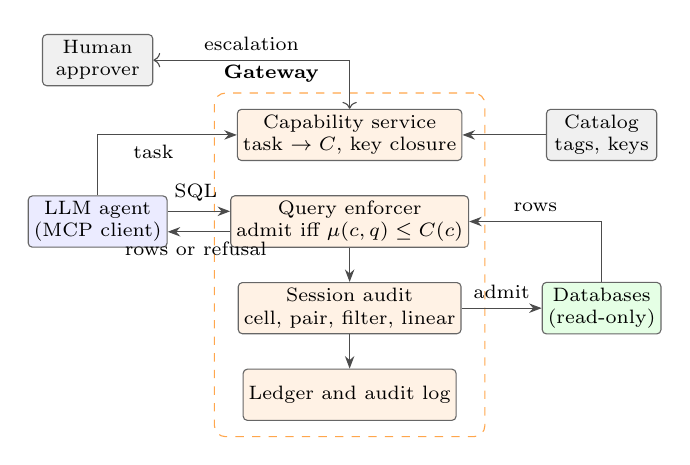
\begin{tikzpicture}[font=\scriptsize,
  box/.style={draw=black!60, rounded corners=1.5pt, fill=#1, minimum height=6.5mm, minimum width=23mm, align=center, inner sep=2pt},
  box/.default=white, side/.style={box=#1, minimum width=14mm},
  arr/.style={-{Stealth[length=1.6mm]}, draw=black!70}]
\node[box=orange!10] (cap) at (0,0) {Capability service\\task $\to C$, key closure};
\node[box=orange!10] (enf) at (0,-1.1) {Query enforcer\\admit iff $\mu(c,q)\le C(c)$};
\node[box=orange!10] (aud) at (0,-2.2) {Session audit\\cell, pair, filter, linear};
\node[box=orange!10] (led) at (0,-3.3) {Ledger and audit log};
\node[draw=orange!70, dashed, rounded corners, fit=(cap)(enf)(aud)(led), inner sep=2mm] (gw) {};
\node[font=\scriptsize\bfseries, anchor=south west] at (gw.north west) {Gateway};
\node[side=blue!8] (agent) at (-3.2,-1.1) {LLM agent\\(MCP client)};
\node[side=gray!12] (human) at (-3.2,0.95) {Human\\approver};
\node[side=green!10] (db) at (3.2,-2.2) {Databases\\(read-only)};
\node[side=gray!12] (cat) at (3.2,0) {Catalog\\tags, keys};
\draw[arr] (agent.north) |- node[pos=0.7, below]{task} (cap.west);
\draw[arr] ([yshift=1.3mm]agent.east) -- node[above, pos=0.45]{SQL} ([yshift=1.3mm]enf.west);
\draw[arr] ([yshift=-1.3mm]enf.west) -- node[below, pos=0.55]{rows or refusal} ([yshift=-1.3mm]agent.east);
\draw[arr] (enf) -- (aud);
\draw[arr] (aud) -- (led);
\draw[arr] (aud.east) -- node[above]{admit} (db.west);
\draw[arr] (db.north) |- node[pos=0.75, above]{rows} (enf.east);
\draw[arr] (cat) -- (cap);
\draw[arr, <->] (cap.north) |- node[pos=0.75, above]{escalation} (human.east);
\end{tikzpicture}
\caption{Gateway between LLM agents and databases. The capability service turns a task into a column-level capability using catalog keys; the enforcer refuses queries that use columns beyond it; the session audit refuses queries whose answer would rest on fewer than $k$ entities given earlier answers; only admitted queries reach the read-only connection. Identifying columns are granted only by a human approver.}
\label{fig:arch}
\end{figure}

\subsection{Session semantics}
A session starts with a purpose, which names the task and the identity it runs under. The gateway issues the capability once per session and keeps three pieces of state for it: the capability, which only grows through escalation; the ledger of entity sets behind admitted answers, per protected column; and the set of entities whose sensitive columns were returned raw, checked against the purpose's entity budget. A refused query changes none of them, because nothing was released.

\subsection{Query pipeline}
Algorithm~\ref{alg:gateway} gives the per-query check. The gateway parses the SQL, resolves every column to $t.c$, checks the capability, runs the audit, and only then executes the query; every decision is logged with the task, the capability and any approval. Sections~\ref{sec:capability} and~\ref{sec:audit} define the two checks.

\begin{algorithm}[!t]
\caption{Gateway check for query $q$ under capability $C$}\label{alg:gateway}
\begin{algorithmic}[1]
\State resolve every column of $q$ to $t.c$; \textbf{if} unresolvable \textbf{return} refuse
\State \textbf{if} $q$ touches a protected or sensitive column inside a CTE, derived table or set operation \textbf{return} refuse
\State $V\gets\{(c,\mu(c,q)):\mu(c,q)>C(c)\}$ \Comment{Eqs.~\ref{eq:mode}--\ref{eq:admit}}
\If{$V\ne\emptyset$} \Return refuse with $V$ (escalation request) \EndIf
\For{$p\in P$ used by $q$ in a filter}
  \State $\mathcal{C}\gets$ candidate sets of the relaxed rewrite; \textbf{if} it fails \textbf{return} refuse
  \If{$\iota_{\downarrow}<k$ \textbf{or} $D_{\downarrow}(q)\ne\emptyset$} \Return refuse \Comment{Eq.~\ref{eq:refuse}} \EndIf
\EndFor
\For{$p\in P$ used by $q$ in mode \textsf{agg}}
  \State $\mathcal{S}\gets$ entity sets of the key-only rewrite; \textbf{if} it fails \textbf{return} refuse
  \If{$\min(\iota_1,\iota_2)<k$ \textbf{or} $D(q)\ne\emptyset$} \Return refuse \Comment{Eq.~\ref{eq:refuse}} \EndIf
\EndFor
\State commit $\mathcal{S}$, $\mathcal{C}$ to $\mathcal{H}$, $\mathcal{H}_{\downarrow}$ and their bases; execute $q$; log
\State \Return rows
\end{algorithmic}
\end{algorithm}

% ─────────────────────────────────────────────────────────────────────────────
\section{Method}\label{sec:method}

\subsection{Mode-aware capabilities}\label{sec:capability}
The idea is to hand the agent the part of the schema its task needs, and to say for each column how it may be used. Counting customers per nation needs the nation key only as a filter; an average balance needs the balance inside an aggregate; only a name the user asked for needs to be returned. The mode in which a query $q$ uses column $c$ is the highest mode over its occurrences $o$:
\begin{equation}\label{eq:mode}
\mu(c,q)=\max_{o\in\mathrm{occ}(c,q)} m(o),
\end{equation}
where $m(o)=\textsf{raw}$ if $o$ is returned (in the outer select list outside any aggregate, or the argument of a projected MIN or MAX), $m(o)=\textsf{agg}$ if $o$ is inside SUM, AVG or another value aggregate, and $m(o)=\textsf{filter}$ otherwise (WHERE, JOIN, GROUP BY, ORDER BY, or inside COUNT). COUNT reveals cardinality, not values; a projected MIN or MAX returns one row's value and is therefore raw. The enforcer admits $q$ under $C$ iff
\begin{equation}\label{eq:admit}
\forall c\in\mathcal{A}:\ \mu(c,q)\le C(c).
\end{equation}
Columns are resolved to $t.c$ by qualifying $q$ against the schema, so aliases, joins and subqueries are handled; a query that cannot be resolved is refused.

\paragraph*{Derivation and key closure} An LLM receives the task, any hint, and the schema with column descriptions, and returns a capability $C_0$ (prompt in the repository). Derived capabilities tend to omit join keys (Section~\ref{sec:rq1}), so the gateway adds, as \textsf{filter}, the keys of the tables $T(C_0)$ that $C_0$ touches:
\begin{equation}\label{eq:closure}
C=C_0\sqcup\{\kappa\mapsto\textsf{filter}:\kappa\in K(T(C_0))\},
\end{equation}
where $\sqcup$ keeps the higher mode per column.

\paragraph*{Escalation} When $q$ violates Eq.~\ref{eq:admit}, the gateway returns the out-of-capability uses $V(q)=\{(c,\mu(c,q)):\mu(c,q)>C(c)\}$. An approver policy may grant them, $C\leftarrow C\sqcup V(q)$. Columns matching a fixed list of identifying attributes (person names, contact, address, birth, gender) are never granted automatically; each becomes a request to a human. The same ceiling applies to $C_0$ itself.

\subsection{Session audit}\label{sec:audit}
The audit asks one question before each query runs: if this answer is released, how few people could it be about, given everything already released? It answers with entity sets. Let $p\in P$ be a protected column of entity table $E(p)$ with key $\kappa$. For an admitted query that aggregates $p$, the gateway rewrites it to select $\kappa$ and the grouping expressions, dropping aggregation, HAVING, ORDER and LIMIT, and runs the rewrite on the read-only connection. This yields $\mathcal{S}(q)=\{S_1,\dots,S_m\}$, one set per output group, and for each a weight vector $w_S$, where $w_S(i)$ is the number of rows entity $i$ contributes to the group. Joins repeat entities: a SUM of balances over \texttt{customer JOIN orders} is $\sum_i w_S(i)\,x_i$ with $w_S(i)$ the customer's order count; without joins every weight is 1. Four tests follow.

\emph{Small cell.} The smallest group rests on
\begin{equation}\label{eq:cell}
\iota_1(q)=\min_{S\in\mathcal{S}(q)}|S|
\end{equation}
entities.

\emph{Nested pair.} With $\mathcal{H}$ the groups of earlier admitted aggregates over $p$, a nested pair reveals the weighted sum over its difference, as in Fig.~\ref{fig:example}a:
\begin{equation}\label{eq:pair}
\iota_2(q)=\min_{(A,B)\in N(q)}\bigl|\{i: w_B(i)>w_A(i)\}\bigr|,
\end{equation}
where $N(q)$ is the set of pairs from $\mathcal{S}(q)\cup\mathcal{H}$ with $w_A\le w_B$ entrywise and $w_A\ne w_B$, at least one of them in $\mathcal{S}(q)$. For unit weights this is $|B\setminus A|$ for $A\subset B$.

\emph{Linear disclosure.} Differences need not be nested. A SUM answer is the inner product of $w_S$ with the vector of per-entity values; an AVG is the same once the group's COUNT is known, which a caller can always obtain. Entity $i$'s value is determined by the answers iff the unit vector $e_i$ lies in their span~\cite{chin1982auditing}. With $Q$ an orthonormal basis of $\{w_S:S\in\mathcal{H}\}$,
\begin{equation}\label{eq:linear}
e_i\in\operatorname{span}(Q)\iff (QQ^{\top})_{ii}=\textstyle\sum_j Q_{ij}^2=1,
\end{equation}
tested with tolerance $10^{-9}$ on normalized weight vectors, and the set of entities $q$ would newly disclose is $D(q)=\{i: (Q'Q'^{\top})_{ii}=1\}$, where $Q'$ extends $Q$ by Gram--Schmidt with $w_S$ for $S\in\mathcal{S}(q)$. The weights are taken only from the bare column: SUM or AVG of an expression of $p$ (a product, a CASE, DISTINCT) is not a weighted sum the audit can model, and is refused.

\emph{Predicate dependence.} A protected column can leak without being aggregated, as Fig.~\ref{fig:example}b shows. When $q$ uses $p$ in its WHERE clause outside any aggregate, the gateway \emph{relaxes} $q$: it replaces every comparison on $p$ with TRUE, which yields a query $q^{\downarrow}$ that matches a superset of $q$'s rows. The candidate sets $\mathcal{C}(q)$ are the entity sets of $q^{\downarrow}$'s output groups, or one singleton per entity if $q$ returns rows rather than aggregates. The answer of $q$ depends on the protected values of these entities and of no others. The gateway applies Eqs.~\ref{eq:cell}--\ref{eq:linear} to $\mathcal{C}(q)$ against a separate history $\mathcal{H}_{\downarrow}$, giving $\iota_{\downarrow}(q)$ and $D_{\downarrow}(q)$. Relaxation gives a superset only for comparisons joined by AND and OR, so a protected column under NOT or CASE, in JOIN ON, GROUP BY, ORDER BY or HAVING, or in a subquery, is refused. So is SUM, AVG, MIN or MAX of a non-protected column under such a filter: summing known, distinct order totals over the customers whose balance passes a threshold would decode which of them passed. Unequal weights decode it too (a \texttt{COUNT(*)} over a join where the target has three orders and two others one each shows whether the target passed), so every candidate in a group must carry the same weight unless the query is \texttt{COUNT(DISTINCT}~$\kappa$\texttt{)}.

The gateway refuses $q$ iff
\begin{equation}\label{eq:refuse}
\min\bigl(\iota_1(q),\iota_2(q),\iota_{\downarrow}(q)\bigr)<k \ \ \text{or}\ \ D(q)\cup D_{\downarrow}(q)\ne\emptyset .
\end{equation}
A refused query reveals nothing, so its sets enter no history. Eq.~\ref{eq:cell} alone is the stateless baseline (cell suppression); Eqs.~\ref{eq:cell}--\ref{eq:pair} form the pairwise audit; Eq.~\ref{eq:refuse} in full is the linear audit.

\paragraph*{Fail-closed coverage} The audit is only as complete as the entity sets it can compute. A protected column referenced inside a CTE, a derived table or a set operation would escape it, because its outer use resolves to the derived relation and the rewrite cannot attribute groups to entities. The gateway therefore refuses any query that touches a protected or sensitive entity column in such a shape, or that references the entity table more than once, and refuses a query whose rewrite fails. A rewrite that succeeds and matches no entity is admitted, since the answer covers no one. Every admitted answer that depends on a protected column has therefore been audited, and every admitted raw return of a sensitive column has been counted against the entity budget.

\paragraph*{Session alarms} For comparison with intent-level monitoring we also compute session scores: drift, the sensitivity-weighted sum $\sum w_c$ over distinct out-of-capability uses $(c,\mu)$, counted once each so that repetition does not grow it; cell, $1/\min(\iota_1,\iota_2)$ over the session; and breadth, the number of distinct entities whose protected or sensitive columns were returned raw, divided by the purpose's entity budget. The gateway also enforces the budget: a query that would return sensitive columns for more entities than the purpose allows is refused.

\subsection{Guarantees}\label{sec:guarantees}
Key closure (Eq.~\ref{eq:closure}) adds only \textsf{filter} modes, so by Eq.~\ref{eq:admit} it never lets a query return or aggregate a column that $C_0$ did not already allow; it widens what a task may join on, not what it may see. For the audit we state the property precisely.

\begin{proposition}\label{prop:linear}
Let $A\in\mathbb{N}^{m\times n}$ have the weight vectors of the $m$ admitted aggregate groups over a protected column as rows, and let each answer be the exact sum $Ax$ of the unknown per-entity values $x\in\mathbb{R}^n$. If no admitted query satisfied $D(q)\ne\emptyset$, then for every entity $i$ and every $x$ there is $x'$ with $Ax'=Ax$ and $x'_i\ne x_i$.
\end{proposition}
\begin{IEEEproof}
Each admission checked Eq.~\ref{eq:linear} with the query's sets added, so after the last admission $e_i\notin\operatorname{row}(A)$ for every $i$; refused queries add no rows. Since $\operatorname{row}(A)=\operatorname{null}(A)^{\perp}$, $e_i\notin\operatorname{row}(A)$ implies some $z\in\operatorname{null}(A)$ has $z_i\ne0$ (otherwise $e_i\perp\operatorname{null}(A)$ and $e_i\in\operatorname{row}(A)$). Put $x'=x+z$. Then $Ax'=Ax$ and $x'_i=x_i+z_i\ne x_i$. The test itself is exact because $(QQ^{\top})_{ii}=\lVert QQ^{\top}e_i\rVert^2$ is the squared norm of the projection of the unit vector $e_i$, which equals 1 iff $e_i$ lies in the span.
\end{IEEEproof}

The predicate test has no such proof, and an exact one is unlikely to be cheap: auditing is hard already for sums of Boolean values~\cite{kleinberg2003boolean}, which is what counts under a threshold are. A count under a threshold is linear in the indicator vector of that threshold, $[x_j>t]_j$, and different thresholds give different unknown vectors. The audit treats all filters on $p$ as one unknown, which refuses every single-entity probe and every nested or linear combination of candidate sets, but an attacker who combines answers across thresholds is not covered by Proposition~\ref{prop:linear}. Strict mode closes that gap.

\paragraph*{Strict mode} Refusals can leak too: the decision depends on which entities match a query, and if membership depends on protected values, a refusal says something about them~\cite{kenthapadi2005simulatable}. In strict mode the gateway refuses any query that uses a protected column outside an aggregate, that is, in WHERE, JOIN, GROUP BY or ORDER BY.

\begin{proposition}\label{prop:strict}
In strict mode, the sequence of gateway decisions for a session is a function of the queries and of the non-protected columns only.
\end{proposition}
\begin{IEEEproof}
Admission under Eq.~\ref{eq:admit} and the strict check depend only on the query text. For an admitted aggregate, the key-only rewrite keeps the query's predicates and groupings and drops its aggregates, so in strict mode it reads no protected column; the entity sets $\mathcal{S}(q)$ and their weights, and hence Eqs.~\ref{eq:cell}--\ref{eq:refuse}, depend only on non-protected data. By induction over the session, $\mathcal{H}$ and $Q$ do too.
\end{IEEEproof}
Refusals in strict mode therefore reveal nothing about protected values beyond what the non-protected columns already reveal, and the threshold probes of Fig.~\ref{fig:example}b never run. The price is refusing legitimate filters on protected values, such as balance bands, which we measure.

\paragraph*{Limits} Proposition~\ref{prop:linear} rules out exact disclosure of one entity's value. For $k>2$ it does not rule out a linear combination of three or more answers that isolates the sum over 2 to $k-1$ entities: Eqs.~\ref{eq:cell}--\ref{eq:pair} catch such small sets only when they appear as a group or as the difference of a nested pair. The audit thus enforces $k$-isolation for groups and nested pairs and exact non-disclosure ($k=1$) for arbitrary linear combinations. It does not rule out narrowing a value to an interval when values are bounded, since $x'$ may fall outside the domain. The small-cell test counts entities, not weight, so a group dominated by one customer's rows passes; dominance rules~\cite{adam1989security} are not applied. Nor does the audit cover values released through non-protected columns, collusion across identities, or, outside strict mode, leakage through refusals themselves~\cite{kenthapadi2005simulatable}.

\subsection{Cost}
Parsing and qualification are linear in the query size. Each rewrite costs one extra query whose result size is the number of matching rows. The linear test keeps $Q\in\mathbb{R}^{n\times r}$ over the $n$ entities touched so far and rank $r\le n$; adding a set costs $O(nr)$ with two Gram--Schmidt passes for stability, and Eq.~\ref{eq:linear} costs $O(nr)$. A query with more groups than a configurable limit (2,000 in our runs) is refused rather than audited. Table~\ref{tab:scaling} measures the check: \Nscalesmallms{} ms with 1,000 entities and rank 10, and \Nscalebigms{} ms with 50,000 entities and rank 500, where the dense basis takes \Nscalebigmb{} MB. Sessions in our workloads stay far below that rank.

\begin{table}[!t]
\caption{Linear-audit check time (median of 5) and basis memory vs.\ entities $n$ and rank $r$, for random contiguous key-range sets (Python/NumPy, Apple M-series CPU, single process on an otherwise idle machine).}
\label{tab:scaling}
\centering\footnotesize
\begin{tabular}{@{}rrrr@{}}
\toprule
$n$ & $r$ & Check (ms) & Basis (MB)\\
\midrule
\tabinput{tables/scaling.tex}
\bottomrule
\end{tabular}
\end{table}

% ─────────────────────────────────────────────────────────────────────────────
\section{Evaluation Methodology}\label{sec:evalmethod}

\subsection{Environment}
Python~3.14, sqlglot~30.23 for parsing and qualification, SQLite and PostgreSQL~16, NumPy, and the MCP Python SDK~2.x. LLMs: gpt-4o-mini and gpt-4o through the OpenAI chat API (temperature 0 for capability derivation and SQL generation; 0.7 with a per-episode seed for attackers), Claude Sonnet 5.5 through the Anthropic API (low effort, provider-side refusal fallback enabled for capability derivation), and qwen3:4b-instruct run locally. All prompts, model outputs and seeds are cached in the repository; every number below is a macro generated from the result files.

\subsection{Data}
\emph{BIRD tasks.} From BIRD dev~\cite{li2023bird} we draw 20 tasks per database from its 11 databases (\Nntasks{} tasks, seed 13); gold SQL and question text are written by BIRD's annotators.
\emph{TPC-H sessions.} A seeded TPC-H-shaped SQLite database (1,500 customers, 7,500 orders, synthetic values) has four purposes and a session generator: \Nnbenign{} benign analyst sessions (400 per purpose) with realistic noise (30\% contain one out-of-purpose query; finance sessions include drill-downs and overlapping histogram bands) and \Nnattack{} attack sessions in five families (drift, small cell, tracker, three-query tracker, enumeration). Every session has 6--16 queries regardless of label, so length carries no label information.
\emph{BIRD sessions.} The human-written gold queries of BIRD's \texttt{financial} (\Nfinnq{} queries) and \texttt{debit\_card\_specializing} (\Ndebitnq{}) databases are arranged into 200 random sessions of 6--16 queries per database.

\subsection{Adaptive attackers}
Each attacker is an LLM told it is red-teaming a privacy gateway over synthetic data and given one customer key; it must find that customer's exact balance in at most 15 queries, seeing rows or refusal reasons after each. Disclosure is decided by an oracle that applies Eq.~\ref{eq:linear} to every answer the gateway returned, independent of what the attacker claims.

\subsection{Statistical reporting}
For a proportion $\hat p$ over $n$ trials we report the 95\% Wilson interval
\begin{equation}\label{eq:wilson}
\frac{\hat p+\frac{z^2}{2n}\pm z\sqrt{\frac{\hat p(1-\hat p)}{n}+\frac{z^2}{4n^2}}}{1+\frac{z^2}{n}},\qquad z=1.96 .
\end{equation}
For paired accuracy differences on the same tasks we report 95\% percentile intervals from 5,000 bootstrap resamples of tasks. Session-alarm thresholds are set per purpose on a held-out half of the benign sessions; detection rates are measured on the other half plus all attacks.

% ─────────────────────────────────────────────────────────────────────────────
\section{Empirical Results}\label{sec:eval}

\subsection{RQ1: Can a task be mapped to a least-privilege capability?}\label{sec:rq1}
Fig.~\ref{fig:captradeoff} places each grant by the columns it exposes and the accuracy of an agent that sees only that grant. With gpt-4o-mini, the role grant exposes \Ncolsmfull{} columns per task and reaches \Nexmfull\% EX. The oracle footprint of the gold query exposes \Ncolsmgold{} columns and reaches \Nexmgold\%, a difference of \NdGoldm\pp{} [\NdGoldmlo, \NdGoldmhi] that includes zero: least privilege is not inherently costly, and narrowing the schema the agent sees does not hurt it. Derivation is where accuracy is lost. The LLM's own column choices fit the gold query in only \Nadmmcols\% of tasks, mostly because join keys are missing, and EX falls to \Nexmcols\%. Key closure (Eq.~\ref{eq:closure}) raises fit to \Nadmmcolskeys\% and EX to \Nexmcolskeys\%. One escalation round, in which \NescRatem\% of tasks request on average \NescReqm{} columns, brings EX to \Nexmesc\% with \Ncolsmesc{} columns: \NdEscm\pp{} [\NdEscmlo, \NdEscmhi] against the role, with a tenth of its columns and about one returnable column per task (\Nrawmcols{}) instead of all of them.

With gpt-4o the pattern holds: role \Nexofull\% EX, oracle footprint \Nexogold\%, derived capability with keys and escalation \Nexoesc\% (\NdEsco\pp{} [\NdEscolo, \NdEscohi] against the role) with \Ncolsoesc{} columns. With Claude Sonnet 5.5 the derived capability costs nothing measurable: \Nexsesc\% against \Nexsfull\% for the role (\NdEscs\pp{} [\NdEscslo, \NdEscshi]) with \Ncolssesc{} columns, and the oracle footprint is clearly more accurate than the role (\Nexsgold\%, \NdGolds\pp{} [\NdGoldslo, \NdGoldshi]). Table~\ref{tab:cap} lists every grant for all four models, including the open-weight qwen3:4b-instruct run locally on a 55-task subset (5 per database; its runtime prevented the full set).

Two observations hold across models. Even the oracle footprint refuses some agent queries (column \emph{Refused}), because the agent often answers correctly with columns other than the gold query's; a capability must allow alternatives rather than one canonical solution. And the cost of a derived capability relative to the role shrinks as the model gets stronger: \NdEscm{} points for gpt-4o-mini, \NdEsco{} for gpt-4o and \NdEscs{} for Sonnet. The weakest model gains from the narrowed schema (role \Nexqfull\%, derived \Nexqesc\%, on 55 tasks with wide intervals), mostly because it writes invalid SQL against 72 columns. The oracle footprint is at least as accurate as the role for every model, so least privilege itself costs nothing; what remains is derivation error, which grows with task difficulty.

\begin{table*}[!t]
\caption{Capability results on \Nntasks{} BIRD tasks. \emph{Admissible}: share of tasks whose gold SQL fits the grant. \emph{EX}: execution accuracy of an agent that sees only the grant [95\% Wilson interval]. \emph{Refused}: share of agent queries the enforcer refuses. \emph{Columns}, \emph{Raw}: mean columns granted, and granted with mode \textsf{raw}. The escalation row grants a refused query's out-of-capability uses once.}
\label{tab:cap}
\centering\footnotesize
\begin{tabular}{@{}llccccc@{}}
\toprule
Model & Grant & Admissible & EX [95\% CI] & Refused & Columns & Raw\\
\midrule
\tabinput{tables/capability.tex}
\bottomrule
\end{tabular}
\end{table*}

Fig.~\ref{fig:capdiff} splits gpt-4o-mini's results by BIRD difficulty: the gap between role and derived capability is about 4 points on simple and moderate tasks and 11 points on the 27 challenging ones, which join more tables, so the derivation misses more of them (the small challenging sample makes this estimate loose).

\begin{figure}[!t]
\centering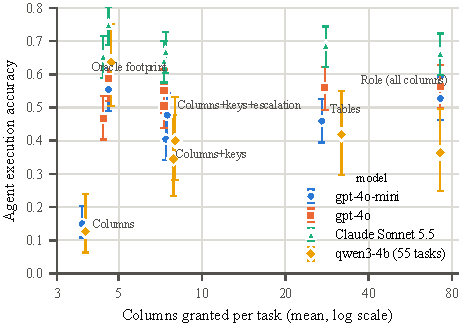
\includegraphics[width=\columnwidth]{figures/fig2_capability_tradeoff.pdf}
\caption{Privilege vs.\ accuracy on \Nntasks{} BIRD tasks. Each point is a grant; $x$: mean columns the agent may use (log scale); $y$: execution accuracy of an agent that sees only those columns; bars: 95\% Wilson intervals. Labels refer to gpt-4o-mini (circles); squares: gpt-4o; triangles: Claude Sonnet 5.5 (all 220 tasks); diamonds: qwen3:4b-instruct (55-task subset).}
\label{fig:captradeoff}
\end{figure}

\begin{figure}[!t]
\centering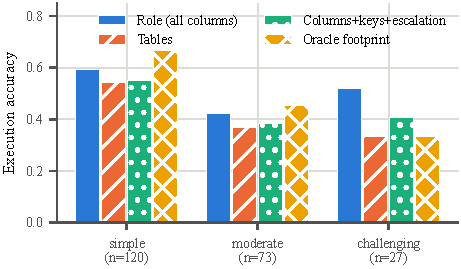
\includegraphics[width=\columnwidth]{figures/fig3_capability_difficulty.pdf}
\caption{Execution accuracy by BIRD difficulty (gpt-4o-mini) for the role grant, table-level grant, derived capability with key closure and one escalation round, and the oracle footprint.}
\label{fig:capdiff}
\end{figure}

\subsection{RQ2: Can the derivation be manipulated?}\label{sec:rq2}
We appended three instructions to each task: a blunt request for all columns, a plausible audit reason asking for names, contact details and birth dates, and an ``admin override'' placed in the hint. Fig.~\ref{fig:inj} reports capability size and the share of tasks whose capability returns identifying columns. For gpt-4o-mini the clean derivation grants \Ninjmcleancols{} columns and identifying columns in \Ninjmcleanident\% of tasks, mostly legitimately, for questions that ask for a person's name. The blunt instruction doubles capability size to \Ninjmbluntcols{} columns; the plausible reason makes \Ninjmplausiblenew\% of tasks gain identifying columns they did not have; the hint injection barely changes anything (\Ninjmhintnew\%). gpt-4o ignores the blunt and hint instructions (\Ninjobluntcols{} and \Ninjohintcols{} columns against \Ninjocleancols{} clean; no new identifying grants) but not the plausible one: \Ninjoplausiblenew\% of tasks gain identifying columns. The stronger model resists crude injection, not plausible text, which is the form real injections take~\cite{greshake2023indirect}.

The approval ceiling stops every injected identifying grant by construction, because no identifying column is granted without a human. Its cost is the clean rate: \Ninjmcleanident\% of clean tasks would wait for approval. It does not bound non-identifying widening, which the blunt injection shows is large.

\begin{figure}[!t]
\centering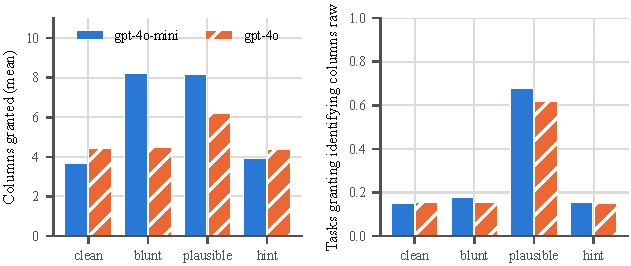
\includegraphics[width=\columnwidth]{figures/fig4_injection.pdf}
\caption{Effect of injected instructions on derived capabilities (\Nntasks{} BIRD tasks). Left: mean columns granted. Right: share of tasks whose capability returns at least one identifying column. \emph{clean}: no injection; \emph{blunt}, \emph{plausible}: appended to the task; \emph{hint}: appended to BIRD's evidence field.}
\label{fig:inj}
\end{figure}

\subsection{RQ3: Which session signals separate attacks from benign work?}\label{sec:rq3}
Fig.~\ref{fig:auroc} gives AUROC for every signal and attack family against held-out benign sessions of the same purpose. Session length carries no label information (query-count AUROC \Naucdriftqueries--\Naucenumerationqueries), so differences are not a length artifact. Each family is separated by the signal that measures its mechanism: drift by out-of-capability use (\Naucdriftdrift), enumeration by breadth (\Naucenumerationbreadth), small cells by the per-query cell test (\Naucsmallcellcellq). The existing SQL guard, which only knows sensitive columns, and the row ledger, which counts sensitive rows, catch enumeration but nothing else.

Fig.~\ref{fig:tpr} shows detection at 1\% benign FPR. Session state helps where the violation is cumulative: drift detection rises from \Ntprstatelessordrift\% to \Ntprstatefulordrift\% (the remainder use only low-sensitivity columns), enumeration from \Ntprstatelessorenumeration\% to \Ntprstatefulorenumeration\%. For the aggregate families, session alarms detect almost nothing at this FPR even though the differencing score ranks trackers well (AUROC \Nauctrackercell). The reason is substantive: \Nbenignleak\% of benign finance sessions (\Nbenignleakn{} of \Nnfinbenign) genuinely isolate one customer, typically an average by nation and segment followed by the same average restricted to positive balances. Honest analysts produce the pattern of Fig.~\ref{fig:example}a too, so an alarm on the session is the wrong tool for this class; the right one refuses the single completing query.

\begin{figure}[!t]
\centering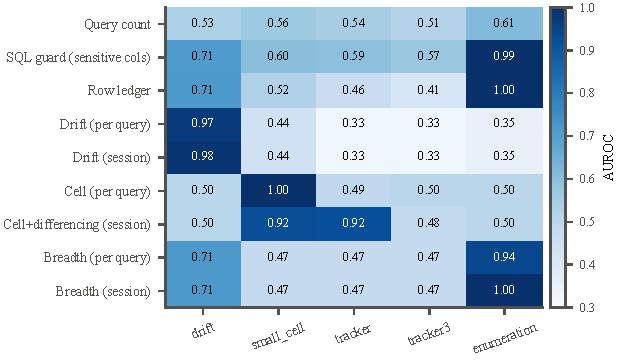
\includegraphics[width=\columnwidth]{figures/fig5_session_auroc.pdf}
\caption{AUROC of each signal (rows) for each attack family (columns) vs.\ held-out benign sessions of the same purpose, on the TPC-H session benchmark (\Nnsessions{} sessions). Per-query signals use the maximum over the session; session signals use accumulated state.}
\label{fig:auroc}
\end{figure}

\begin{figure}[!t]
\centering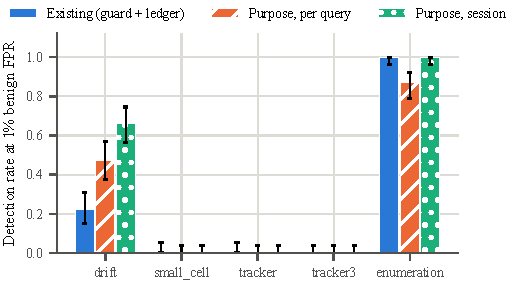
\includegraphics[width=\columnwidth]{figures/fig6_session_tpr.pdf}
\caption{Detection rate of session alarms at a 1\% target benign FPR (thresholds per purpose on held-out benign sessions; OR detectors split the budget across their three signals). Bars: 95\% Wilson intervals over 100 attack sessions per family.}
\label{fig:tpr}
\end{figure}

\subsection{RQ4: What does query-level auditing prevent, and at what cost?}\label{sec:rq4}
The audit refuses only the query that would complete an isolation (Eq.~\ref{eq:refuse}). Fig.~\ref{fig:audit} plots attacks prevented against benign finance queries refused. Cell suppression alone (stateless) refuses \Nrefkthreestateless\% of benign queries at $k=3$ but prevents only \Nprevkthreestatelesstracker\% of trackers. The pairwise audit prevents \Nprevkthreepairwisetracker\% of trackers at \Nrefkthreepairwise\% benign refusals, but only \Nprevkthreepairwisetrackerthree\% of three-query attacks whose sets are not nested. The linear audit prevents \Nprevkthreelineartracker\% of trackers and \Nprevkthreelineartrackerthree\% of three-query attacks at the same benign cost as the pairwise audit (\Nrefkthreelinear\% of queries; \Nhitkthreelinear\% of benign sessions see at least one refusal). The linear test adds protection without adding benign refusals, because honest workloads rarely produce exact linear dependencies that the small-group and pairwise tests do not already catch. Strict mode keeps the same protection (\Nprevkthreestricttracker\% and \Nprevkthreestricttrackerthree\%) but refuses \Nrefkthreestrict\% of benign queries, because analysts filter on balances (histogram bands, drill-downs above a threshold); simulatable decisions cost this much on our workload. At $k=5$ every non-strict mode refuses \Nrefkfivelinear\% of benign queries, because ordinary nation-by-segment groupings contain fewer than five customers.

\paragraph*{Threshold probes} The bisection of Fig.~\ref{fig:example}b aggregates no balance, and without the predicate test it passes every other test: against the linear audit on TPC-H, 21 counts of the form \texttt{COUNT(*) WHERE c\_custkey = 570 AND c\_acctbal > $t$} recovered the target's balance to the cent with no refusal. With the predicate test the first probe is refused, since its candidate set holds one customer. \emph{Join fan-out.} An earlier, unweighted version fell to two probes from an independent review. Sixteen admitted SUMs over \texttt{customer JOIN orders} in date windows where customers have different order counts, plus those counts, determined customer 570's balance within 227 queries, in strict mode too, since the weights depend only on orders; a \texttt{COUNT(*)} bisection over a window where the target has three orders and two others one each recovered it in 21 probes. With weights, the first attack leaves the value undetermined after 1{,}192 queries (334 refused); the equal-weight rule refuses the second at its first probe.

All benign rates in this section include the predicate test and the weights; the histogram bands and drill-downs of the finance sessions pass it because their candidate sets are whole nation-by-segment groups.

\paragraph*{Comparison with differential privacy} Instead of refusing, a gateway could answer every aggregate over the protected column with Laplace noise~\cite{dwork2006calibrating,johnson2018flex}. We clip balances to $[-1{,}000,10{,}000]$ (sensitivity 10,000 per SUM), split a session budget $\varepsilon$ equally across its protected aggregates, and answer an average as a noisy sum over the exact group size. Table~\ref{tab:dp} compares utility on the benign finance sessions with the share of tracker sessions in which the attacker's estimate lands within 10\% of the target's balance. At $\varepsilon=10$, benign answers are off by a median of \Ndptenmed\% and only \Ndptenfive\% are within 5\%, while the attacker succeeds in \Ndptenatt\% of sessions; at $\varepsilon=100$, \Ndphundredfive\% of benign answers are within 5\% but the attacker succeeds in \Ndphundredatt\%. On groups of about a dozen customers no budget gives both. The audit instead refuses \Nrefkthreelinear\% of benign queries and returns the rest exactly. To score it by the same criterion, we give the attacker every exact answer the linear audit admitted in each tracker session (as group sums) and solve two linear programs for the lowest and highest balance of the target consistent with them and with the clipping domain; the attacker's estimate is the midpoint. That estimate is within 10\% of the target's balance in \Ndpauditatt\% of the \Ndpauditn{} sessions, the same rate as guessing the midpoint of the domain with no answers at all (\Ndpauditprior\%), and the admitted answers narrowed the target's interval in \Ndpauditnarrowed{} of them. Against that reference, the DP attacker gains over guessing only at $\varepsilon=100$; at smaller budgets its noisy estimate is worse than the guess, so its rates below \Ndpauditprior\% mean no gain, not added protection. The comparison is not one-sided: differential privacy bounds inference for every query and needs no entity sets, while the audit's result holds for these attacks and this domain, not as a general bound. Differential privacy suits large groups and approximate dashboards; the audit suits exact answers over small groups.

\begin{table}[!t]
\caption{Differential privacy vs.\ the session audit on the finance workload. \emph{Median error}, \emph{Within 5\%}: relative error of benign answers per output group. \emph{Refused}: benign queries refused. \emph{Attacker}: share of tracker sessions whose estimate is within 10\% of the target's balance (audit: midpoint of the linear-programming bound; guessing the domain midpoint scores \Ndpauditprior\%).}
\label{tab:dp}
\centering\footnotesize
\setlength{\tabcolsep}{3.5pt}
\begin{tabular}{@{}lcccc@{}}
\toprule
Answering & Median error & Within 5\% & Refused & Attacker\\
\midrule
\tabinput{tables/dp.tex}
Linear audit, $k=3$ & 0 & 100\% & \Nrefkthreelinear\% & \Ndpauditatt\%\\
\bottomrule
\end{tabular}
\end{table}

\begin{figure}[!t]
\centering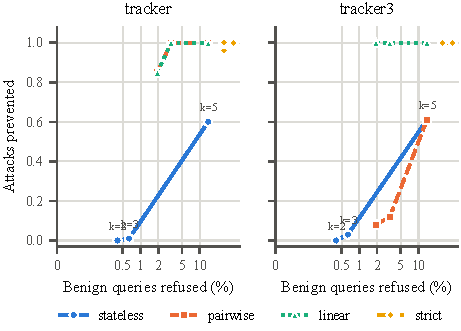
\includegraphics[width=\columnwidth]{figures/fig7_audit_tradeoff.pdf}
\caption{Query-level audit on finance sessions: share of attacks prevented (refused at or before the disclosing query) vs.\ share of benign queries refused, for $k\in\{2,3,5\}$ and the four audit modes (strict: linear plus no predicates on the protected column). Left: two-query trackers; right: three-query trackers whose sets are not nested. $x$ axis symmetric-log.}
\label{fig:audit}
\end{figure}

\subsection{RQ5: Does the audit hold against adaptive attackers?}\label{sec:rq5}
We ran \Nadvnm{} targets per defense with gpt-4o-mini and \Nadvno{} with gpt-4o (the gpt-4o strict-mode run and its extension to 50 targets were not completed). Claude Sonnet 5.5 declined the attacker role on the first turn of every episode, so it contributes no attacker data. Fig.~\ref{fig:adaptive} reports oracle disclosure. With column rules only, both attackers succeed almost always (gpt-4o-mini \Nadvmpurpose\%, gpt-4o \Nadvopurpose\%), usually with one AVG over a single key. Cell suppression stops direct isolation but not differencing (\Nadvmstateless\%, \Nadvostateless\%). The pairwise audit is defeated by combinations it does not model; the disclosed episodes include overlapping key ranges such as $[570,577]+[577,590]-[570,590]$ and equal-size averages over shifted key triples, neither of which contains a nested pair differing by fewer than three entities (\Nadvmpairwise\%, \Nadvopairwise\%). gpt-4o-mini had three \texttt{UNION ALL} queries answered unaudited in runs that predate the fail-closed rule, two in one pairwise-audit episode and one in a column-rules-only episode; removing them from the answered sets leaves both targets disclosed, so those rates are unchanged, and no such query was answered under the linear or strict audit. Under the linear audit no target was disclosed by either attacker (0 of \Nadvnm{} and 0 of \Nadvno{}; upper 95\% bounds \Nadvmlinearhi\% and \Nadvolinearhi\%), at \Nadvmlinearrefusals{} and \Nadvolinearrefusals{} refusals per episode. Strict mode gives \Nadvmstrict\% disclosure for gpt-4o-mini, with refusals that by Proposition~\ref{prop:strict} carry no information about balances.

These episodes were run before the predicate test existed, and the oracle measures exact linear disclosure only. No attacker tried a threshold bisection; had one done so, the oracle would not have counted it. The predicate test only adds refusals, so the linear-audit result stands, and the threshold channel is covered by the scripted probe in Section~\ref{sec:rq4} rather than by these runs.

\begin{figure}[!t]
\centering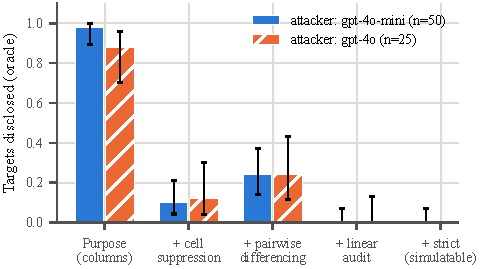
\includegraphics[width=\columnwidth]{figures/fig8_adaptive_attacker.pdf}
\caption{Adaptive LLM attackers: share of targets whose exact balance is determined by the answers the gateway returned (oracle, Eq.~\ref{eq:linear}), per defense and attacker model. Bars: 95\% Wilson intervals.}
\label{fig:adaptive}
\end{figure}

\subsection{RQ6: Cost on human-written queries and overhead}\label{sec:rq6}
The TPC-H workloads above are generated. Fig.~\ref{fig:bird} uses BIRD's human-written queries instead, with an analytics purpose that permits every column except per-entity amounts and balances, which may only be aggregated. On \texttt{financial}, \Nfinmode\% of queries return a protected value raw and are refused by the capability; the full audit refuses \Nfinreflinear\%, against \Nfinrefstateless\% for per-query suppression. On \texttt{debit\_card\_specializing} the figures are \Ndebitmode\%, \Ndebitreflinear\% and \Ndebitrefstateless\%. Strict mode refuses \Nfinrefstrict\% and \Ndebitrefstrict\%. The high rate on \texttt{debit\_card\_specializing} reflects its questions, many of which ask for one customer's consumption; under an aggregate-only purpose those are disclosures by design, so the rate measures policy fit, not audit error.

Most of the audit's refusals on \texttt{financial} come from the predicate test, and they are disclosures the aggregate tests alone admitted. Taken one at a time in a fresh session, \Nfinsingle{} of its queries are refused, against \Nfinsingleold{} without the predicate test. Of these, \Nfincatrank{} rank accounts by a protected value (\texttt{ORDER BY amount DESC LIMIT 1}, ``which account has the largest loan''), which names the entity at the top, and \Nfincatthreshold{} list the accounts whose amount passes a threshold, which reveals one bit of each listed account's value. On \texttt{debit\_card\_specializing}, \Ndebitcataggregate{} of its \Ndebitsingle{} single-query refusals are per-customer aggregates. The multiplicity rules of Sec.~\ref{sec:audit} cost \Nfincatfanout{}+\Nfincatexpression{} and \Ndebitcatfanout{}+\Ndebitcatexpression{} queries: protected-filter \texttt{COUNT}s over joins (rewritable with \texttt{COUNT(DISTINCT} key\texttt{)}) and conditional sums such as \texttt{SUM(IIF(CustomerID = 7, Consumption, 0))}, which can single out one entity; rewriting \texttt{SUM(CASE WHEN $p$ THEN $x$ ELSE 0 END)} as a filtered sum would admit the benign ones. In both databases the stateful tests (nested pairs, linear combinations) refused nothing the per-query tests had not: on human-written sessions the audit costs only its per-query rules. The aggregate rewrite computed entity sets for \Nfincov\% and \Ndebitcov\% of the protected aggregates; the fail-closed rule refuses the rest (CTEs, nested set operations), so they count as refusals rather than as unaudited answers.

The monitor's median check takes \Nfinlatmed{} and \Ndebitlatmed{} ms, against \Nfinqmed{} and \Ndebitqmed{} ms for the queries themselves; at the 95th percentile, \Nfinlatp{} and \Ndebitlatp{} ms against \Nfinqp{} and \Ndebitqp{} ms. Overhead is dominated by the key-only rewrite, which scans as many rows as the query.

\begin{figure}[!t]
\centering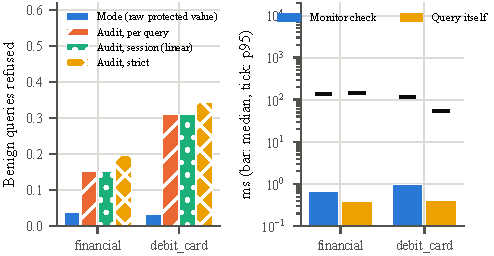
\includegraphics[width=\columnwidth]{figures/fig9_bird_benign.pdf}
\caption{Human-written BIRD workloads (200 sessions per database). Left: share of benign queries refused by the capability (raw protected value), by per-query cell suppression, and by the full session audit, $k=3$. Right: monitor check time vs.\ the query's own execution time (bars: median; ticks: 95th percentile; log scale).}
\label{fig:bird}
\end{figure}

\subsection{RQ7: Does it work as an MCP gateway at scale?}\label{sec:rq7}
We loaded the TPC-H-shaped schema into PostgreSQL~16 at roughly scale factor 1 (150,000 customers, 1.5M orders, 4.5M line items; the gateway connects through a role with only SELECT and a read-only transaction default). We generated \Neesessions{} sessions against this database (40 benign per purpose, 20 per attack family; \Neequeries{} queries), transpiled them to PostgreSQL, and replayed them through an MCP client on two paths: the gateway executing on Postgres itself, and the gateway forwarding to a separate database MCP server that holds the database connection, as an existing vendor server would. Table~\ref{tab:e2e} reports the results.

Both paths reproduced the in-process library's decision on every query (\Needirparity\% parity, no errors), so the protocol layer neither drops nor alters decisions. Every attack in all five families was refused at or before its disclosing query (drift at the column check, enumeration by the entity budget), while \Needirbenlo--\Needirbenhi\% of benign queries per purpose were refused, mostly out-of-purpose slips. The median gateway check took \Needirchkmed{} ms against a median query execution of \Needirexmed{} ms, and MCP transport added about \Needirtr{} ms. The tail is the key-only rewrite: at the 95th percentile the check took \Needirchkp{} ms, for aggregates whose rewrite returns every matching customer key; through the proxy, those keys also cross a second MCP hop (\Neeprxchkp{} ms). Computing entity sets inside the database, for example as a hashed bitmap, would remove the shipping of keys.

\begin{table}[!t]
\caption{End-to-end MCP deployment on PostgreSQL at TPC-H scale factor $\approx$1 (\Neesessions{} sessions, \Neequeries{} queries). \emph{Parity}: decisions equal to the in-process library. Times in ms, median / 95th percentile; \emph{Transport}: round trip minus check and execution, median.}
\label{tab:e2e}
\centering\scriptsize
\setlength{\tabcolsep}{2.5pt}
\resizebox{\columnwidth}{!}{%
\begin{tabular}{@{}lccccc@{}}
\toprule
Path & Parity & Check & Execute & Transport & Round trip\\
\midrule
\tabinput{tables/e2e.tex}
\bottomrule
\end{tabular}}
\end{table}

% ─────────────────────────────────────────────────────────────────────────────
\section{Enterprise Readiness}\label{sec:enterprise}
In an enterprise the gateway sits as an MCP proxy in front of database MCP servers, so agents and databases are unchanged; Section~\ref{sec:rq7} shows this path works without changing decisions. The capability for a task is issued once and carried with the session, and the human approval step attaches to the identity the application authenticates. Because the gateway sees every source an agent queries, the ledger can extend across databases, where linkage between, for example, customer and payroll systems is invisible to each system's own policy. Capabilities can also be compiled into native views and row policies as a second line of enforcement. Table~\ref{tab:checklist} lists what a deployment has to decide.

\begin{table}[!t]
\caption{Deployment checklist.}
\label{tab:checklist}
\centering\footnotesize
\begin{tabular}{@{}p{0.3\columnwidth}p{0.62\columnwidth}@{}}
\toprule
Item & Decision\\
\midrule
Database account & SELECT-only role, read-only transaction default\\
Catalog & Entity tables and keys; sensitivity tag per column\\
Protected columns & Which per-entity values may only be aggregated\\
Identifying columns & List reviewed against catalog tags; named approver\\
Audit mode & $k$; linear (exact filters allowed) or strict (simulatable refusals)\\
Entity budgets & Per purpose, for tasks that need individual records\\
Decision log & Retention and who may read it\\
\bottomrule
\end{tabular}
\end{table}

\paragraph*{Where it adds little} For agents that already act strictly as the end user through narrow APIs, the remaining gain is the session audit. Tasks that legitimately need individual records, such as a support agent helping one customer, need a purpose with an entity budget rather than an aggregate-only rule; the breadth signal covers that case, but its budget is a policy choice.

% ─────────────────────────────────────────────────────────────────────────────
\section{Discussion}\label{sec:discussion}

\subsection{Metric limitations}
Execution accuracy compares result sets and ignores answers that are correct in substance but differ in form, which affects every grant equally. The adaptive-study oracle counts only exact linear disclosure; it does not count interval narrowing or threshold bisection, which the scripted probe covers instead. The DP comparison scores both arms by a within-10\% estimate built from the answers and the clipping domain alone; an attacker who knows the distribution of balances would do better against both.

\subsection{Threats to validity}
Capability derivation was measured with three commercial models on 220 tasks and one open-weight model on 55; the injection study covers only the two OpenAI models. The TPC-H sessions and attack families are authored by us; the adaptive study and the BIRD workloads reduce, but do not remove, this dependence. The identifying-column list is a fixed name rule that both over- and under-matches. The audit does not stop inference of bounds or collusion across identities, and only strict mode removes leakage through refusals; differential privacy~\cite{dwork2006calibrating,johnson2018flex} addresses some of these at the price of exact answers. Overhead was measured on SQLite (up to about one million rows) and on PostgreSQL at TPC-H scale factor 1; warehouse engines and larger scales remain untested.

\subsection{Next steps}
The next concrete step is to compute entity sets inside the database as hashed bitmaps, which removes the tail latency of Section~\ref{sec:rq7} and lets the predicate test keep one basis per threshold instead of one for all. After that: a per-task escalation budget to bound non-identifying widening, an interval oracle for the adaptive study, and evaluation on logged, consented enterprise sessions.

% ─────────────────────────────────────────────────────────────────────────────
\section{Conclusion}\label{sec:conclusion}
We built an MCP gateway that gives each agent task a column-level, mode-aware capability and audits every answer that depends on a protected column against the entity sets of earlier answers. Capabilities removed about nine tenths of the columns an agent could use while execution accuracy changed by between \NdEscs{} and \NdEscm{} points across models, and the audit stopped every scripted and adaptive differencing attack while refusing \Nrefkthreelinear\% of benign generated queries. It deploys in front of an existing database MCP server unchanged and keeps exact answers for queries that single no one out.

\section*{Data and Code Availability}
Code, prompts, LLM caches, generators and results are in the author's repository; BIRD is not redistributed, and the TPC-H-shaped database is regenerated from a seed.

\section*{Declarations}
\textbf{Funding, conflicts of interest, use of AI tools:} [to be completed by the author, per the journal's policy].

\bibliographystyle{IEEEtran}
\bibliography{references}

\end{document}
